\documentclass[11pt,a5paper]{article}

\usepackage[T1]{fontenc}
\usepackage[utf8]{inputenc}
\usepackage{lmodern, microtype}
\usepackage[estonian]{babel}
\usepackage{siunitx}
\sisetup{inter-unit-product=\ensuremath{{}\cdot{}}, per-mode=fraction, exponent-product=\cdot, output-decimal-marker={,}}
\usepackage{graphicx}
\usepackage{wrapfig}
\usepackage{adjustbox}
\usepackage{tikz}
\usetikzlibrary{arrows.meta, patterns, patterns.meta}
\usepackage{pgfplots}
\usepackage[european]{circuitikz}
\tikzset{component/.style={draw,thick,circle,fill=white,minimum size=0.75cm,inner sep=0pt}}
\usepackage{amsmath,amssymb}
\usepackage{amsfonts}
\usepackage[hidelinks]{hyperref}
\usepackage{csquotes}
\usepackage{caption}
\usepackage{enumitem}
\topmargin=-3.0cm \textheight=19cm \textwidth=12.9cm
\oddsidemargin=-1.5cm  \evensidemargin=-1.5cm
\setlength{\parindent}{0pt} \setlength{\parskip}{6pt} \sloppy
\sloppy \relpenalty=10000 \binoppenalty=10000
\pagestyle{empty}

\newcommand{\numb}[1]{\vspace{5pt}\textbf{\large #1}}
\newcommand{\nimi}[1]{(\textsl{\small #1})}
\newcommand{\punktid}[1]{(\emph{#1~p.})}
\newcounter{ylesanne}
\newcommand{\yl}[1]{\addtocounter{ylesanne}{1}\numb{\theylesanne.} \nimi{#1} \newblock{}}
\newcommand{\autor}[1]{}% Kasuta võistluse ajal
%\newcommand{\autor}[1]{\emph{Autor: #1}}% Kasuta kui vaja autorit

\begin{document}
\begin{center}
  \textbf{\Large Eesti koolinoorte 69. füüsikaolümpiaad} \par
  \emph{9. aprill 2022. a. lõppvoor\\Gümnaasiumi ülesanded (10.--12. klass)}
\end{center}

\resizebox{\textwidth}{!}{
  \emph{%
    \begin{tabular}{@{}l@{}}
      \textbf{Palun kirjutada iga ülesande lahendus eraldi lehele.}\\
      Lahendamisaeg on 5 tundi. Iga osavõtja võib lahendada kõiki pakutud ülesandeid. \\
      Arvesse lähevad 5 suurima punktide arvu saanud teoreetilist ja 1 eksperimentaalne ülesanne. \\
      Kasutada võib kirjutus- ja joonestusvahendeid ning kalkulaatorit. Muud abivahendid on keelatud.\\
      Eksperimentaalülesande lahendamisel võib kasutada üksnes loetelus toodud vahendeid. \\
      Mõõtemääramatuse hindamist ei nõuta.
    \end{tabular}
  }
} \par

\yl{KETTAHEIDE}
Taganttuul on spordis harilikult abiks, kuid mitte kettaheites. Selgitage kvalitatiivselt, miks vastutuul võib suurendada kettaheite tulemust. Visandage joonis, kus lendav ketas on kujutatud vertikaalläbilõikes näidates seal ketta lennusuuna ja tuule suuna. Näidake sellel joonisel jõudiagrammina, millised jõud mõjuvad kettale lennu ajal ja kirjeldage, kuidas mõjutab neid jõude vastutuul.
\punktid{6} \autor{Jaan Kalda}

\yl{LUMEVÄLI}
Mari on kooli hiljaks jäämas ning proovib välja arvutada, kuidas joosta üle kooli ees oleva väljaku, mis on lumega kaetud. Väljak on ristkülikukujuline, mille ühes tipus asub Mari ja diagonaali teises tipus koolimaja uks. Väljaku koolimaja fassaadiga parallelne külg on \SI{100}{\metre} pikk ja koolimajaga risti olev külg \SI{50}{\metre}. Mari jookseb mööda teed kiirusega \SI{6}{\metre\per\second}, ja ta hindab, et ta jookseb lumes 20\% aeglasemalt kui mööda väljaku ääres olevat teed. Kui palju aega on võimalik Maril säästa joostes üle lumise väljaku võrreldes sellega, kui ta jookseks mööda väljaku ääres olevat teed?
\punktid{8} \autor{Moorits Mihkel Muru}

\begin{wrapfigure}{r}{5cm}
  \vspace{-2em}
  \begin{center}
    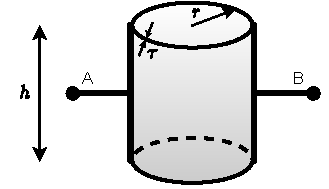
\includegraphics[width=\linewidth]{silinder.pdf}
  \end{center}
  \vspace{-2em}
\end{wrapfigure}

\yl{SILINDER} Õhukese silindri eritakistus on $\rho$, raadius on $r$, kõrgus on $h$ ja paksus on $\tau$. Silindri ringikujulised põhjad on eemaldatud ning silindri vastaspooltel on silindri materjal asendatud peenikeste juhtivate klemmidega, mille pikkus on $h$ ja paksus on $\tau$ (A ja B joonisel). Leidke kahe klemmi vaheline takistus.
\punktid{8} \autor{Richard Luhtaru}


\yl{LÄÄTSEDE KOLMNURK}
Kuhu tuleb paigutada ekraan, et ekraanile tekiks kaks valgusallika $A$ kujutist? Kolme läätse fookused ühtivad ja asuvad punktis $F$. Lahendage ülesanne lisalehel.
\punktid{8} \autor{Erkki Tempel}
\newpage

\yl{JALGRATAS}
Elektrijalgratta mootor asub ratta rummus ning suudab arendada maksimaalset pöördemomenti $M=\SI{60}{\newton\meter}$ ja maksimaalset kasulikku võimsust $P=\SI{500}{W}$ (võib eeldada, et viimane ei sõltu kiirusest). Rattad on 26-tollised ehk raadiusega $r=\SI{0.33}{m}$. Jalgratta ja sõitja summaarne mass $m=\SI{110}{kg}$. Hõõrdejõu rataste telgedes võib lugeda tühiseks. \\
\osa Kui suure maksimaalse tõusunurgaga mäenõlvast saaks sellise jalgrattaga vaid elektri jõul üles sõita? \\
\osa Kui suure maksimaalse kiiruse saavutaks jalgratas mõne aja möödudes, kui tõus oleks $\alpha=\SI{5}{\degree}$? \punktid{8} \autor{Valter Kiisk}

\yl{ÕHUPÜSS}
Õhupüssis kasutatakse rõhu $p_1=\SI{34}{MPa}$ all olevat lämmastikku kuuli kiirendamiseks. Milline on püssirauda jääva lämmastiku temperatuur vahetult peale lasku? Enne lasku oli surulämmastik toatemperatuuril $t_0=\SI{20}\celsius$; õhurõhk $p_0=\SI{100}{kPa}$. Lämmastiku molaarne soojusmahtuvus konstantsel ruumalal on $c_V=\frac 52R$ ja keemistemperatuur $T_k=\SI{-196}\celsius$. \\
\textit{Vihje:} Helikiirusest aeglasemates protsessides gaasiga, kus ei toimu soojusvahetust, kehtib nn adiabaadiseadus $pV^\gamma=const$, kus lämmastiku jaoks on astmenäitaja $\gamma=7/5$. 
\punktid{10} \autor{Jaan Kalda}

\yl{VEEUPUTUS}
Tänava kanalisatsioon on ehitatud selliselt, et vihmasaju korral koguneb vihmavesi kõigepealt tänava all kulgevasse kraavi, kust omakorda juhitakse vesi ära sadeveetorustiku kaudu. Sadeveetorustiku ummistuse tõttu suudab see aga tagada sadevee äravoolu ainult 50\% võimsusel maksimaalsest võimalikust. Ükskord paduvihma ajal juba 6 minutit peale vihma algust sai kraav täis ning vesi tungis tänavale. Graafikul (pöördel) on toodud sademete koguhulga $h$ sõltuvus ajast $t$ alates paduvihma algusest. \\
Peale paduvihma lõppemist tehtud arvutused näitasid, et isegi juhul, kui sadeveetorustik poleks ummistunud, poleks see uputusest päästnud ning kraav oleks täitunud 9 minutit peale vihma algust.\\
Milline pidanuks olema töökorras torustiku äravoolu minimaalne võime (liitrit minutis $\SI{1} {m^2}$ pinna kohta), et uputust ei oleks tekkinud? \punktid{10} \autor{Oleg Ko\v sik}

\yl{VEEVALAJA}
Oleg seisab kaalul ja ta ühes käes on pudel, kus on $m=\SI{1}{\kilogram}$ vett ja teises käes on piisavalt suur anum, mis on $h=\SI{1}{\meter}$ madalamal kui pudel. Ta hakkab pudelist vett välja valama anumasse kiirusega $\dot{m}=\SI{1}{\kilo\gram / \second}$.
Joonistage graafik (koos arvulise skaalaga), kuidas muutub kaalu näit alates hetkest, kui kogu vesi on veel pudelis kuni hetkeni, kui kogu vesi on jõudnud anumasse. Raskuskiirendus on $g=\SI{10}{\meter / \second\squared}$ ja võib eeldada, et vesi liigub pudelist anumasse ilma õhutakistuseta. Anum on nii lai, et veenivoo seal ei muutu. Tehtud arvutused koos põhjendustega kirjutage eraldi lehele.
\punktid{12} \autor{Kaur Aare Saar}

\newpage

\yl{SATELLIIT}
Millise temperatuuri omandab väike kuubikujuline absoluutselt must satelliit, mis liigub Maa ümber madalal ringorbiidil (kõrgus maapinnast on hulga väiksem, kui Maa raadius) ja on parajasti öö külje peal. \\
Vihje: Maad võib vaadelda kui lõpmatut tasandit, mis on temperatuuril $T_0=\SI{15}\celsius$ ja omab kiirgustegurit $\epsilon=\num{0.6}$, st tema soojuskiirgustihedus ($\SI{}{\watt / \metre\squared}$) on 60\% samasuguse absoluutselt musta keha soojuskiirgustihedusest $\sigma T^4$, kus $\sigma$ tähistab Stefan‐Boltzmanni konstanti.
\punktid{12} \autor{Jaan Kalda}

\yl{PLAAT}
Väike ringikujuline laenguta metallist plaat raadiusega $r$ ja paksusega $h$ asetati plaadi teljel olevast punktlaengust $q$ kaugusele $R$. Hinnake, millise jõuga $F$ tõmbub või tõukub plaat laengu poole. Võite eeldada, et $h\ll r\ll R$ ja plaadi keskme ning ääre juurde indutseeritud laengute tõttu tekkinud jõud on tühiselt väike. 
\punktid{12} \autor{Konstantin Dukats}

\end{document}

